\section{Régulateur PID}

\subsection{Introduction}

Afin de réguler les variations en sortie $PV$, on utilise un régulateur PID, qui reprend la valeur de $PV$ pour la soustraire à la consigne $SP$ donnant donc l'erreur $E = SP - PV$ à corriger sur $MV$.\\
Pour rappel, un régulateur PID est composé de trois termes:
\begin{itemize}
    \item Le terme proportionnel $P$ qui est proportionnel à l'erreur $E$ et vise une erreur statique nulle.
    \item Le terme intégral $I$ qui est proportionnel à la somme des erreurs passées et donc accumule l'erreur.
    \item Le terme dérivé $D$ qui est proportionnel à la dérivée de l'erreur et vise à corriger anticipativement l'erreur future.
\end{itemize}
La sortie du régulateur est alors donnée par :
\begin{equation}\label{eq:PID}
    MV = K_C \, \left( 1 + \frac{1}{T_I s} + \frac{T_D s}{\alpha T_D s + 1}\right) \, E
\end{equation}

Dans le cadre du laboratoire, le régulateur utilise également le \textbf{Reset de l'Action Intégrale} et la \textbf{Saturation de l'Action Intégrale} venant adapter l'action intégrale en fonction de, respectivement, la valeur de $MV$ en mode manuel, et la saturation de $MV$ atteignant les limites $MV_{MAX}$ / $MV_{MIN}$.
\begin{center}
    $MV_I = MV_{Man} - MV_P - MV_D - MV_{FF}$\\[4pt]
    et\\[4pt]
    $MV_I = MV_{MAX} - MV_P - MV_D - MV_{FF}$
\end{center}

Afin de pouvoir implémenter le régulateur PID, toutes les formules ont évidemment été discrétisées, et ce pour deux méthodes : Euler Backwards Difference (EBD) et Trapezoïdes (TRAP).

\subsection{Optimisation par la méthode IMC}

Il est important de choisir les paramètres $K_C$, $T_I$ et $T_D$ de façon à implémenter le bon régulateur pour notre processus.
Une façon d'obtenir ces paramètres optimaux est de réaliser un step sur $MV$ et d'observer la dynamique du Processus.
Le modèle trouvé va nous permettre de calculer ces valeurs via des tables.\\
On utilisera la ligne I du tableau présent dans le cours, correspondant à un modèle du second ordre avec délai ($\tau_3 = 0$).
\begin{align*}
    K_C &= \frac{1}{K_P} \, \frac{T_{1p} + T_{2p}}{T_{CLP} + \theta}\\[4pt]
    T_I &= T_{1p} + T_{2p}\\[4pt]
    T_D &= \frac{T_{1p} \, T_{2p}}{T_{1p} + T_{2p}}
\end{align*}
Il est bon de noter que nous aurions pu utiliser la ligne G du tableau (premier ordre avec délai) totalement équivalente étant donné que notre Processus est du premier ordre ($T_{2p} \approx 0$).
La constante $T_D$ et donc l'action Dérivée valant 0, le regulateur devient enfait un régulateur PI.
\begin{align*}
    K_C &= \frac{1}{K_P} \, \frac{T_{1p}}{T_{CLP} + \theta}\\[4pt]
    T_I &= T_{1p}\\[4pt]
    T_D &= 0
\end{align*}
La constante de temps en boucle fermée $T_{CLP}$ est un certain ratio de la première constante de temps du processus $T_{1p}$ définit par $T_{CLP} = \gamma \, T_{1p}$. L'influence de $\gamma$ sera discuté en simulation de boucle fermée par après.

\subsection{Réponse indicielle du régulateur PID}

Nous allons maintenant analyser la réponse du régulateur lorsqu'on applique une erreur $E$ constante à son entrée.
La figure \ref{fig:Step_Response_PID} représente cette réponse.
\begin{figure}[h]
    \centering
    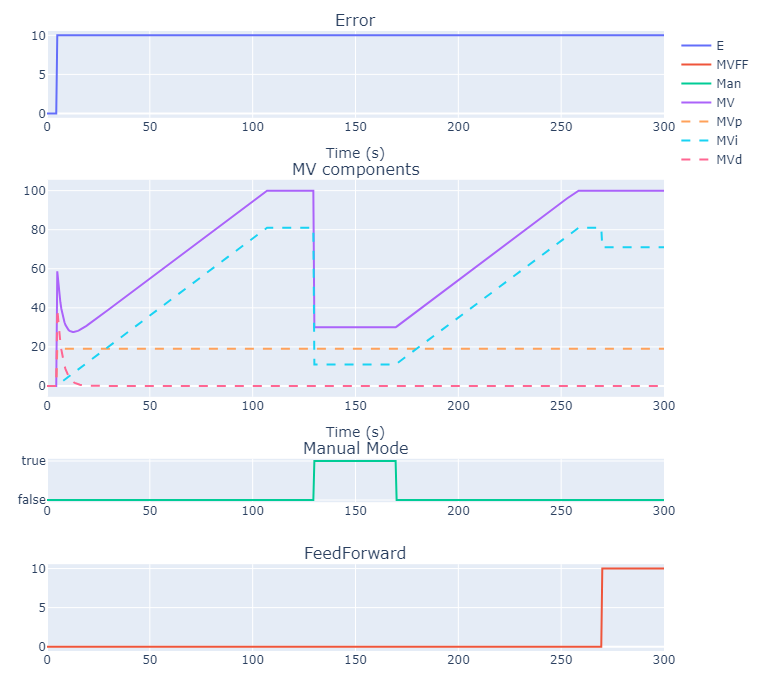
\includegraphics[width=0.8\textwidth]{../Plots/PID/PID_Response_error_step.png}
    \caption{Réponse indicielle du PID à un step sur E ($K_C = 1.9$, $T_D = 6$, $T_I = 24$, $\alpha = 0.4$)}
    \label{fig:Step_Response_PID}
\end{figure}
Premièrement, nous voyons tout au long du graphique que $MV$ est la somme de ces actions $MV = MV_P + MV_I + MV_D + MV_{FF}$.
A l'instant du step sur l'erreur, la composante proportionnelle $MV_P$ augmente instantanément puisqu'elle est proportionnelle à l'erreur, la composante intégrale $MV_I$ est encore nulle puisqu'elle n'a pas encore accumulé d'erreurs, et la composante dérivée $MV_D$ est limitée à $1/\alpha$ puis diminue suivant sa constante de temps $T_D$.

Ensuite, lorsque nous sommes en mode automatique, l'action intégrale $MV_I$ augmente linéairement puisque l'erreur est constante.
Cela va continuer jusqu'à éventuellement atteindre les limites imposées sur la sortie $MV$, ici, une puissance de chauffe $MV_{MAX} = 100\%$ et $MV_{MIN} = 0\%$.
Il est alors nécessaire de réaliser un Reset de l'Action Intégrale, c'est-à-dire, venir adapter la valeur de $MV_I$ pour garder la sortie $MV$ dans les limites.
\begin{equation*}
    MV_I = MV_{MAX} - MV_P - MV_D - MV_{FF}
\end{equation*}

Lorsque l'on passe en mode manuel (boucle ouverte), la valeur de $MV$ est donnée par l'opérateur et donc ici, fixé à 30\%.
En effet, on voit sur le graphe que $MV$ chute à 30\% et que l'action intégrale $MV_I$ est alors adaptée pour garder la sortie $MV$ à cette valeur.

Enfin, une perturbation à été ajoutée à la fin de la simulation pour montrer l'effet de l'action Feed-Forward.
À saturation, le Reset de l'Action Intégrale prends également en compte cette perturbation pour garder la sortie $MV$ dans les limites et donc, on le voit sur le graphe lorsque $MV_I$ est réduit de 10\%.
Si $MV$ ne sature pas, cette perturbation sera directement ajoutée à la sortie $MV$ permettant ainsi de minimiser l'impact sur $PV$.

\subsubsection{Influence de \texorpdfstring{$K_C$}{Kc}}
\begin{figure}[H]
    \centering
    \begin{subfigure}[b]{0.48\textwidth}
        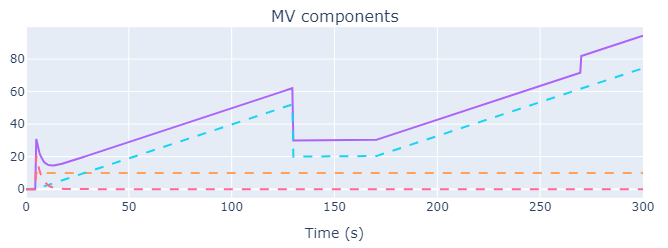
\includegraphics[width=\textwidth]{../Plots/PID/PID_Response_low_Kc.png}
        \caption{$K_C = 1$}
    \end{subfigure}
    \begin{subfigure}[b]{0.48\textwidth}
        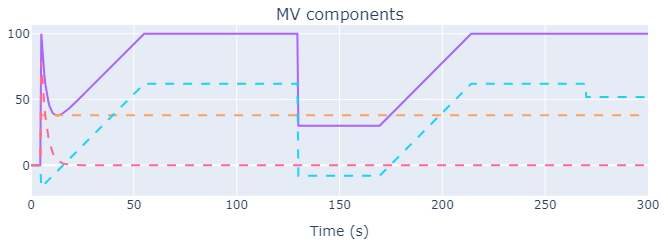
\includegraphics[width=\textwidth]{../Plots/PID/PID_Response_high_Kc.png}
        \caption{$K_C = 3.8$}
    \end{subfigure}
    \caption{Influence de $K_C$ sur la réponse indicielle du PID}
    \label{fig:Kc_Influence_PID}
\end{figure}
Le gain du régulateur $K_C$ est un gain, donc un multiplicateur agissant sur toutes les actions comme le montre l'équation \eqref{eq:PID}.
On voit sur la Figure \ref{fig:Kc_Influence_PID} que pour $K_C = 1$, tout est atténué et nous atteignons même pas la saturation.
Une perturbation en fin de simulation est alors ajoutée à $MV$ et non enlevée à $MV_I$ pour conserver $MV_{MAX}$ sur $MV$.

Lorsque l'on augmente $K_C$, tout est amplifié et plus aggressif. On le voit directement avec l'atteinte rapide de la saturation.
Un gain trop élevé peut poser problème puisque le pic initial de l'action dérivée est directement proportionnel à $K_C$.
Le graphe (b) montre même une saturation de ce pic obligeant l'action intégrale $MV_I$ à passer en négatif.\\
Nous pouvons également faire le lien avec le coefficient $\gamma$. Celui-ci agit directement sur le gain sortant de l'optimisation IMC via la relation de la ligne I du tableau.
\begin{equation*}
    K_C = \frac{1}{K_P} \, \frac{T_{1p} + T_{2p}}{\gamma \, T_{1p} + \theta}
\end{equation*}
Il est clair que pour un processus et délai fixe, un grand $K_C$ induit un petit $\gamma$ et donc un caractère plus aggressif du régulateur.

\subsubsection{Influence de \texorpdfstring{$T_D$}{Td} et \texorpdfstring{$T_I$}{Ti}}
\begin{figure}[H]
    \centering
    \begin{subfigure}[b]{0.48\textwidth}
        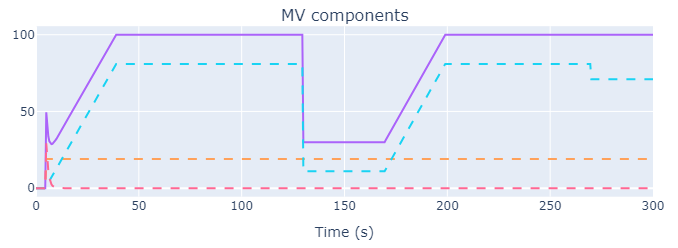
\includegraphics[width=\textwidth]{../Plots/PID/PID_Response_low_Td.png}
        \caption{$T_D = 2\,s$ ($T_I = 8\,s$)}
    \end{subfigure}
    \begin{subfigure}[b]{0.48\textwidth}
        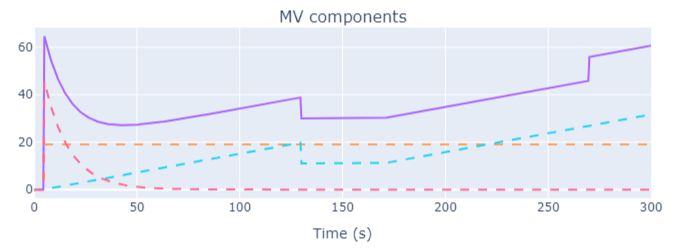
\includegraphics[width=\textwidth]{../Plots/PID/PID_Response_high_Td.png}
        \caption{$T_D = 30\,s$ ($T_I = 120\,s$)}
    \end{subfigure}
    \caption{Influence de $T_D$ et $T_I$ sur la réponse indicielle du PID}
    \label{fig:Td_Influence_PID}
\end{figure}
La constante de temps dérivée agit sur la pente de la tangente initialeet donc aussi sur le temps de montée de l'action dérivée.
La constante de temps intégrale agit sur la pente de l'action intégrale.
Étant donné que l'on respecte généralement $\frac{T_D}{T_I} < 0.25$, nous avons choisi de limiter les constantes par $T_I = \frac{T_D}{0.25}$.

Nous constatons effectivement que l'action dérivée atteint son régime établi bien plus rapidement lorsque $T_D = 2\,s$ que lorsque $T_D = 30\,s$.
Il y a également une différence notable quant à la hauteur du pic initial de l'action dérivée. Elle est représentée par :
\begin{equation*}
    MV_D = K_C \, E \, \frac{T_D s}{\alpha T_D s + 1}
\end{equation*}
Travaillant à une fréquence suffisement grande, lorsque 1 est non-négligeable par rapport à $\alpha T_D$, le pic est influencé par $T_D$.
Arrivé à une valeur de $T_D$ suffisement grande, le 1 devient négligeable, et $T_D s$ peut se simplifier résultant en un pic qui tends vers :
\begin{equation*}
    MV_D = \frac{K_C \, E}{\alpha} = \frac{1.9 \cdot 10\%}{0.4} = 47.5\%
\end{equation*}
En effet, le graphe (b) montre déjà un pic de 45.6\% pour $T_D = 30\,s$ rendant celui-ci presque indépentant à une augmentation de $T_D$.

La Figure \ref{fig:Td_Influence_PID} montre également l'impact de $T_I$ sur la pente de l'action intégrale.
Cette action intégrale est inversemment proportionnelle à $T_I$.
\begin{equation*}
    MV_I = \frac{K_C \, E}{T_I s}
\end{equation*}
L'accumulation de l'erreur aura donc une plus grande valeur pour une constante $T_I$ plus faible, résultant en une variation plus grande de $MV_I$, en d'autres termes, une pente plus élevée.

\subsubsection{Influence de \texorpdfstring{$\alpha$}{alpha}}
\begin{figure}[H]
    \centering
    \begin{subfigure}[b]{0.48\textwidth}
        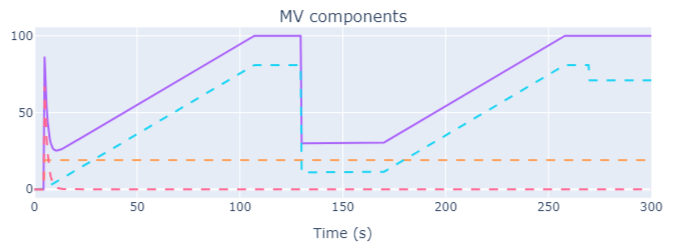
\includegraphics[width=\textwidth]{../Plots/PID/PID_Response_low_alpha.png}
        \caption{$\alpha = 0.2$}
    \end{subfigure}
    \begin{subfigure}[b]{0.48\textwidth}
        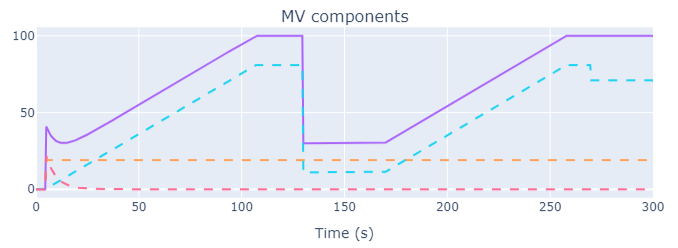
\includegraphics[width=\textwidth]{../Plots/PID/PID_Response_high_alpha.png}
        \caption{$\alpha = 0.8$}
    \end{subfigure}
    \caption{Influence de $\alpha$ sur la réponse indicielle du PID}
    \label{fig:Alpha_Influence_PID}
\end{figure}
Le coefficient $\alpha$ est tout bonnement ce qui va permettre de limiter le gain en hautes fréquences, donc en somme, le pic initial sur l'action dérivée.
Le dérivateur est enfait $MV_D = T_D s$ qui est impropre, puisqu'à hautes fréquences, $s$ tend vers l'infini. Un filtre du $1^{er}$ ordre est alors appliqué avec un ratio de la constante de temps $T_D$.
\begin{align*}
    &MV_D = K_C \, E \, (T_D s)\\
    \Longrightarrow \quad &MV_D = K_C \, E \, \frac{T_D s}{\alpha T_D s + 1} \, \longrightarrow \, \frac{K_C \, E}{\alpha}
\end{align*}
Nous voyons sur la Figure \ref{fig:Alpha_Influence_PID} que le pic est effectivement plus grand pour un $\alpha$ plus petit, et vice-versa.

\subsection{FeedForward}

\begin{figure}[h]
    \centering
    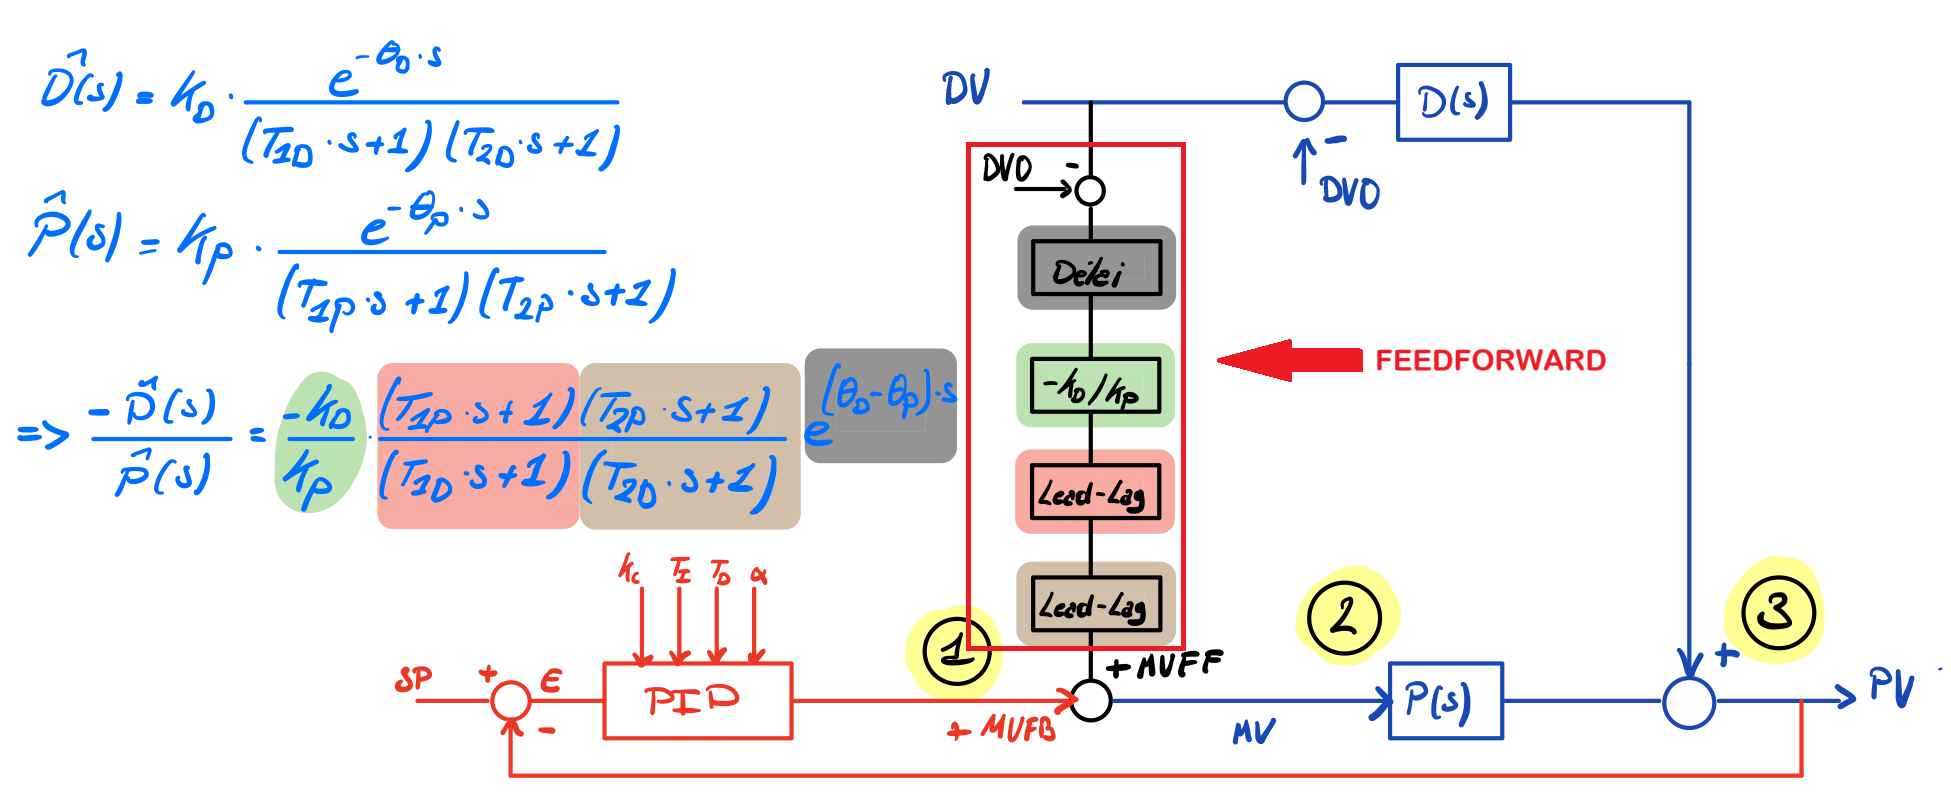
\includegraphics[width=\textwidth]{figures/schemaFF.png}
    \caption{Schema du régulateur PID avec fonction de FeedForward}
	\label{fig:schemaFF}
\end{figure}

La fonction de FeedForward est conçue pour anticiper et compenser l'impact des perturbations ($DV$) sur la variable du processus ($PV$), 
avant que ces dernières n'affectent le système.
\\Le fonctionnement du FeedForward peut être décrit de manière mathématique comme suit : 
\begin{itemize}
	\item 
	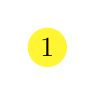
\begin{tikzpicture}
		\fill[fill=yellow!80!] (0,0) circle [radius=0.25cm];
		\node at (0,0) {1};
	\end{tikzpicture} Premièrement, la valeur manipulée en sortie du PID, $MV_{FB}$, est ajustée par une valeur $MV_{FF}$, calculée pour compenser directement la perturbation :
	\begin{equation} \label{eq:1}
		MV_{FF} = K_{FF}\cdot\frac{(T_{1P}s + 1)(T_{2P}s + 1)}{(T_{1D}s + 1)(T_{2D}s + 1)}\cdot e^{-\theta_{FF}}\,DV = \frac{\hat{D}(s)}{\hat{P}(s)}\,DV
	\end{equation}
	où : 
	\begin{equation}\label{eq:2}
		K_{FF} = \frac{K_D}{K_P},
	\end{equation}
	\begin{equation}\label{eq:3}
		\theta_{FF} = |\theta_D - \theta_P|
	\end{equation}
	\item 
	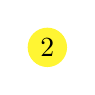
\begin{tikzpicture}
		\fill[fill=yellow!80!] (0,0) circle [radius=0.25cm];
		\node at (0,0) {2};
	\end{tikzpicture}Ensuite, après la sortie du n\oe{}ud $MV = MV_{FB} - MV_{FF}$, on obtient : 
	\begin{equation}\label{eq:4}
		P(s)\cdot MV \approx P(s)\cdot MV_{FB} - \hat{D}(s)
	\end{equation}
	\item
	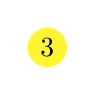
\begin{tikzpicture}
		\fill[fill=yellow!80!] (0,0) circle [radius=0.25cm];
		\node at (0,0) {3};
	\end{tikzpicture} Pour enfin arriver au n\oe{}ud final où l'on additionne la dynamique de la perturbation $D(s)$ à celle du processus : 
	\begin{equation}\label{eq:5}
		P(s)\cdot MV_{FB} - \hat{D}(s) + D(s) \approx P(s)\cdot MV_{FB} = PV
	\end{equation}
\end{itemize}
\subsubsection{Délai}

La $1^{ère}$ étape dans la réalisation de la fonction du FeedForward est de récupérer la perturbation $DV$, de la ramener au point de fonctionnement et de lui appliquer un délai $\theta_{FF}$ (\ref{eq:3}).
L'application de ce délai se fait à l'aide de la fonction \texttt{Delay\_RT} :
\begin{python*}
	Delay_RT(self.DV - self.DV0*np.ones_like(self.DV), # On recentre DV sur le point de fonctionnement
		max(self.theta_ODV_SOPDT-self.theta_OMV_SOPDT, 0), # Calcul du délai 
		self.Ts, 
		self.MVFF_Delay)
\end{python*}

\subsubsection{Gain et Lead-Lag}
Après avoir appliqué le délai à la perturbation et l'avoir recentrée pour la ramener au point de fonctionnement, l'étape suivante
consiste à appliquer le gain (\ref{eq:2}) et le premier Lead-Lag.
\\Ajouter un signe négatif au gain puis additionner le $MV_{FF}$ au $MV_{FB}$ ou laisser le gain positif et soustraire $MV_{FF}$ au $MV_{FB}$ est sans conséquences sur le système.
\\Le premier Lead-Lag dont $T_{Lead} = T_{1P}$ et $T_{Lag} = T_{1D}$ couplé au gain et au délai permet d'obtenir la fonction de transfert : 
\[K_{FF}\, \frac{T_{1P}s + 1}{T_{1D}s + 1} \, e^{\theta_{FF}}\]
Pour se faire, on utilise la fonction \texttt{LL\_RT} sur le signal $DV$ retardé et centré (\texttt{MV\_Delay}) via : 
\begin{python*}
	LL_RT(self.MVFF_Delay, 
		-self.Kp_ODV_SOPDT/self.Kp_OMV_SOPDT, # gain
		self.T1_OMV_SOPDT, #TLead
		self.T1_ODV_SOPDT, #TLag
		self.Ts, 
		self.MVFF_LL1)
\end{python*}
On applique ensuite un second Lead-Lag afin d'obtenir la fonction de transfert complète (\ref{eq:1}) dont la
constant $T_{Lead} = T_{2P}$ et $T_{Lag} = T_{2D}$.
\\Dans le cas où le FeedForward est désactivé, on applique un gain nul au second Lead-Lag donc $MV_{FF} = 0$ : 
\begin{python*}
	if self.FF == True:
		LL_RT(self.MVFF_LL1, 
			1, # Gain unitaire quand le FeedForward est activé
			self.T2_OMV_SOPDT, #TLead
			self.T2_ODV_SOPDT, #TLag
			self.Ts, 
			self.MVFF
		)
	else:
		LL_RT(self.MVFF_LL1, 
			0, # Gain nul quand le FeedForward est désactivé
			self.T2_OMV_SOPDT, 
			self.T2_ODV_SOPDT, 
			self.Ts, 
			self.MVFF
			) 
\end{python*}




